\documentclass[11pt]{article}

\usepackage[margin=1in]{geometry}
\usepackage[T1]{fontenc}
\usepackage{lmodern}
\usepackage{microtype}
\usepackage{amsmath,amssymb,amsthm,mathtools}
\usepackage{graphicx}
\usepackage[dvipsnames]{xcolor}
\usepackage{booktabs}
\usepackage{hyperref}

\hypersetup{
  colorlinks=true,
  linkcolor=MidnightBlue,
  citecolor=MidnightBlue,
  urlcolor=MidnightBlue
}

\newtheorem{theorem}{Theorem}
\newtheorem{proposition}{Proposition}
\newtheorem{remark}{Remark}

\newcommand{\Tmax}{T}

\title{\textbf{Eliminative Information in a Generalized Monty Hall Problem II}\\
\large Variable Reveal Costs, Interior Optima, and Learning Curves}
\author{}
\date{}

\begin{document}
\maketitle

\begin{abstract}
Part I studied the generalized Monty Hall problem with a constant cost per
host reveal and found an exact endpoint threshold: reveal everything if
$c<1/K$ and reveal nothing if $c>1/K$.  This second note keeps the same
eliminative-information mechanism but allows reveal costs to vary with the
number of reveals already purchased.  The probability of success after $t$
reveals remains
\[
  S(t)=\frac{m(K-1)}{K(K-1-t)},
\]
but the objective becomes $S(t)-C(t)$ for a cumulative cost curve $C$.
The stopping rule is governed by the comparison
\[
  S(t+1)-S(t) \quad \hbox{versus} \quad c_t.
\]
Linearly increasing costs can create genuine interior optima, so the clean
endpoint theorem is not robust to arbitrary learning-cost curves.  Costs that
rise and then saturate partly restore the Part I ``push-through'' phenomenon:
late eliminative information can again dominate early unattractive steps.
\end{abstract}

\section{The Baseline Carried Forward}

There are $K$ doors and $m$ prizes, with $1\le m<K$.  The player chooses one
door, and a knowledgeable host can reveal losing doors, never opening a prize
or the player's initial door.  After $t$ reveals the player switches uniformly
among the remaining non-initial closed doors.

The maximum number of possible reveals is
\[
  \Tmax=K-m-1.
\]
The switch success probability is
\[
  S(t)=\frac{m(K-1)}{K(K-1-t)},\qquad 0\le t\le \Tmax.
\]
Its one-step gain is
\[
  \Delta_t=S(t+1)-S(t)
  =
  \frac{m(K-1)}{K(K-2-t)(K-1-t)},
  \qquad 0\le t<\Tmax.
\]
The important inherited fact is that $\Delta_t$ is strictly increasing.
Eliminating a losing door is more valuable when the candidate set is already
small.

\section{Variable Reveal Costs}

Let $c_t\ge0$ be the cost of buying reveal $t+1$, after $t$ reveals have
already been purchased.  Define
\[
  C(t)=\sum_{i=0}^{t-1} c_i,\qquad C(0)=0.
\]
The variable-cost stopping problem is
\[
  \max_{0\le t\le \Tmax} W(t),
  \qquad
  W(t)=S(t)-C(t).
\]

\begin{proposition}[Increment rule]
The net increment from buying one more reveal is
\[
  W(t+1)-W(t)=\Delta_t-c_t.
\]
\end{proposition}

\begin{proof}
This follows directly:
\[
  W(t+1)-W(t)
  =
  S(t+1)-S(t)-\{C(t+1)-C(t)\}
  =
  \Delta_t-c_t.
\]
\end{proof}

Thus variable costs create a competition between two sequences: the increasing
benefit sequence $\Delta_t$ and the cost sequence $c_t$.

\begin{figure}[ht]
  \centering
  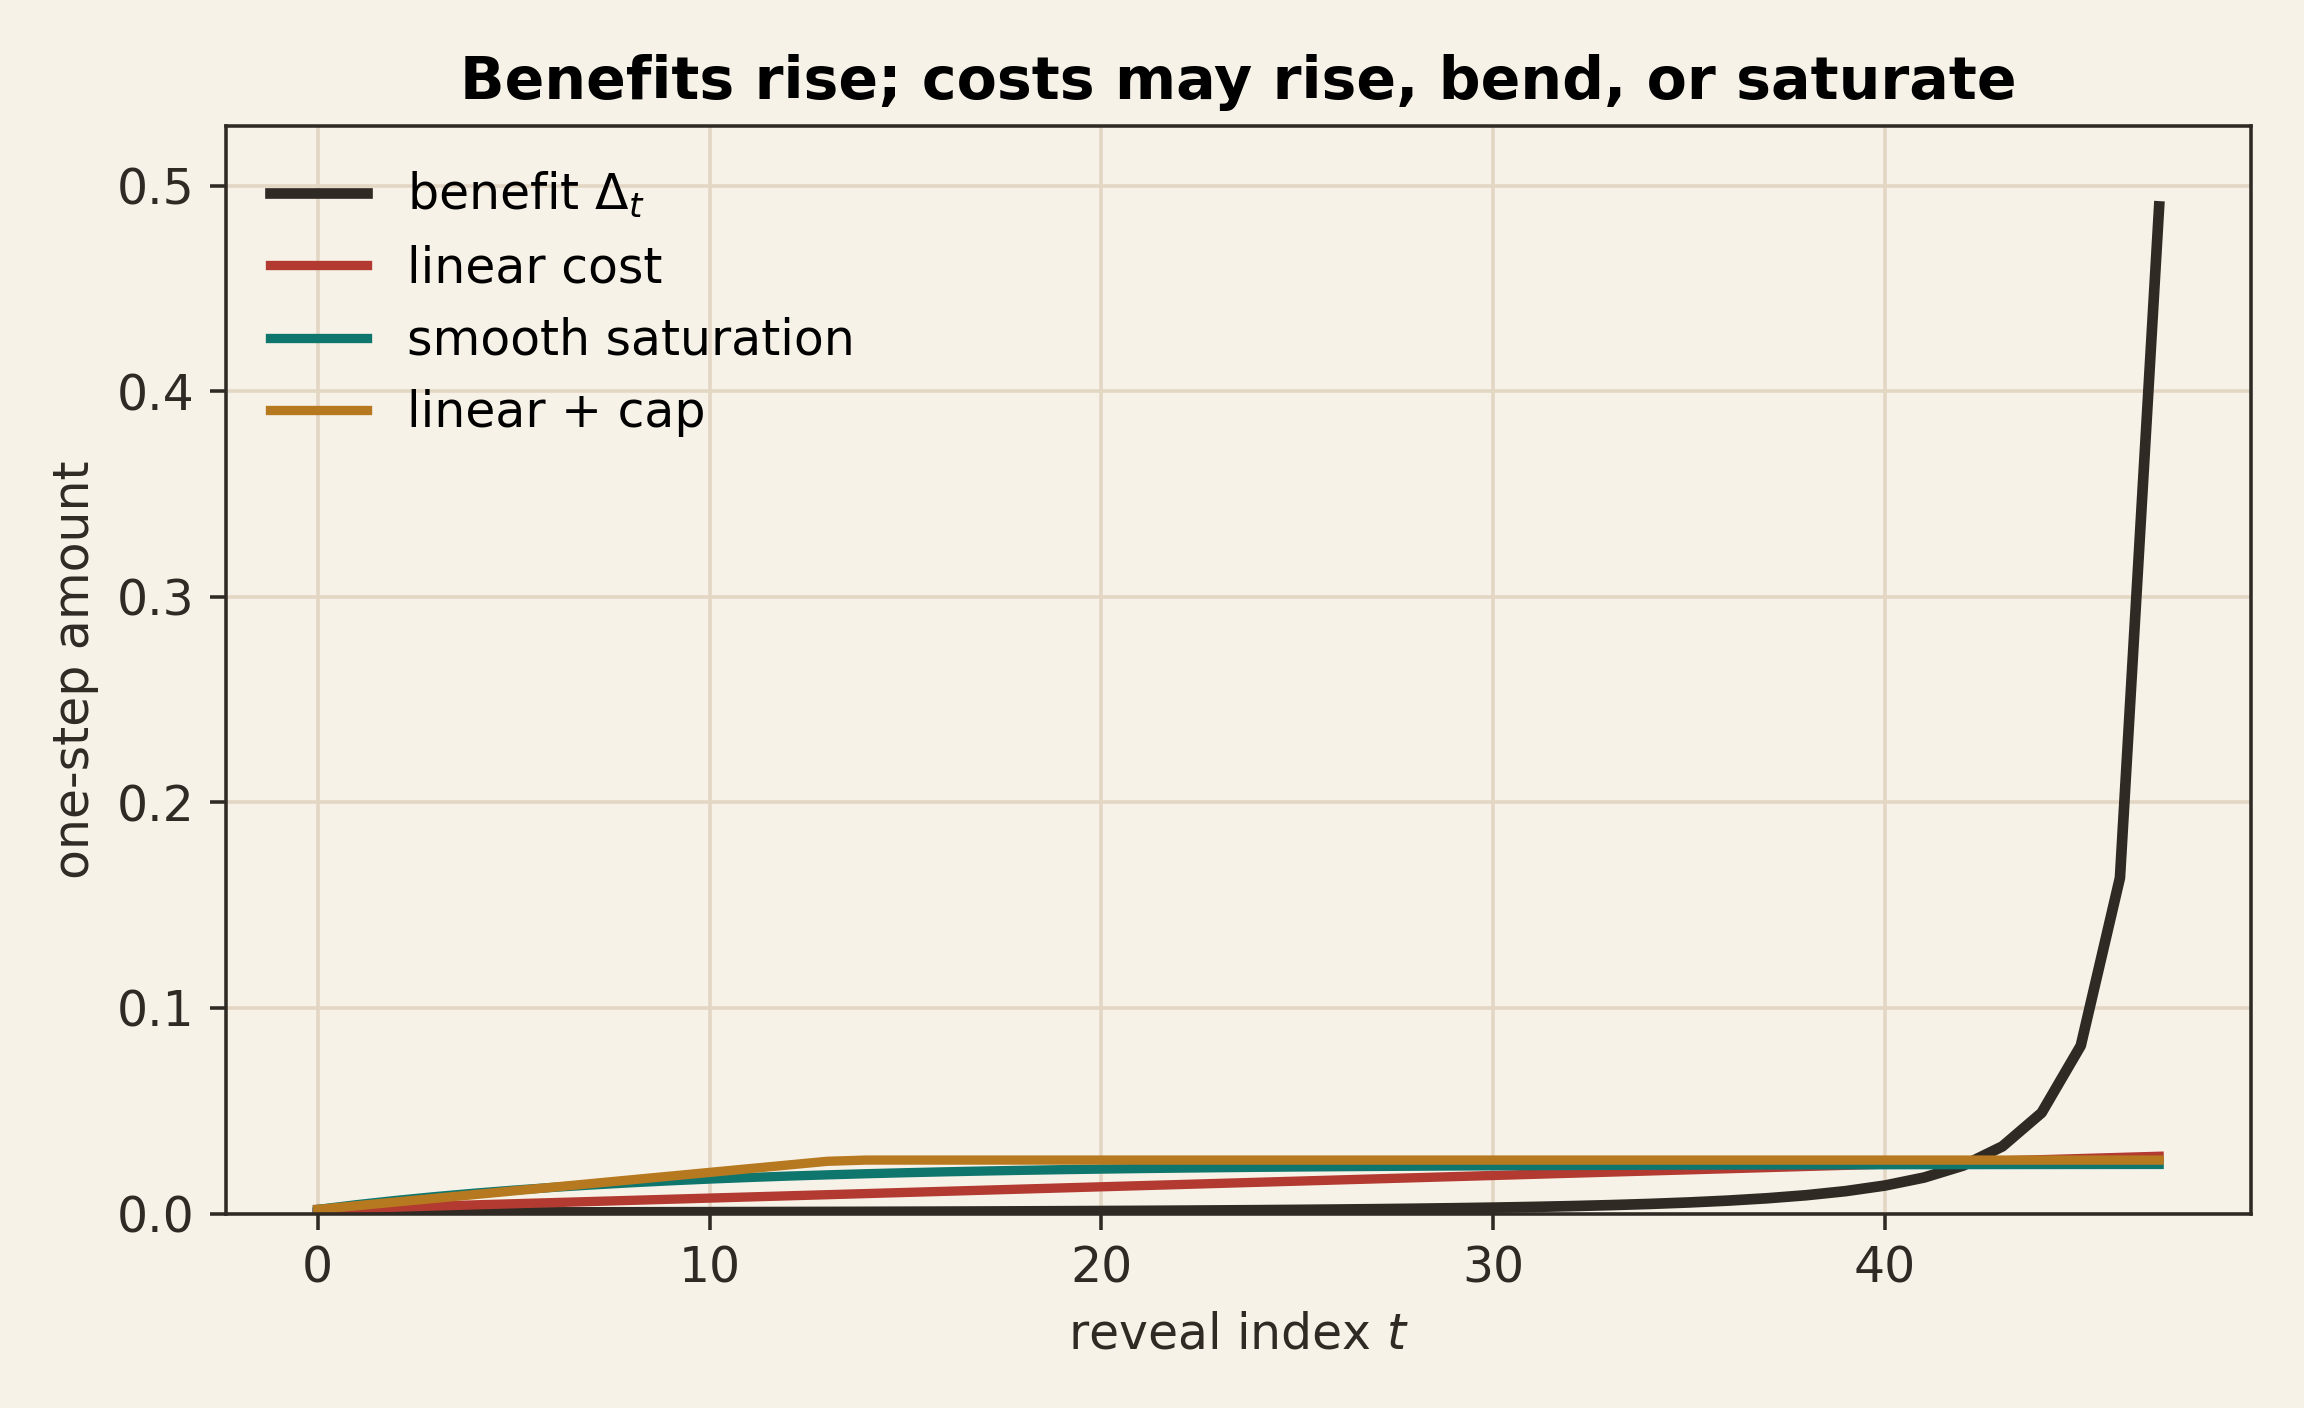
\includegraphics[width=0.88\linewidth]{fig_cost_shapes.png}
  \caption{For $K=50,m=1$, the eliminative-information benefit $\Delta_t$
  rises sharply near the end.  Different learning-cost curves interact with
  this same benefit curve in different ways.}
  \label{fig:cost-shapes}
\end{figure}

\section{What Constant Costs Hid}

In Part I, $c_t=c$ for every $t$.  Since $\Delta_t$ is increasing, the
increments $\Delta_t-c$ are also increasing.  Therefore $W$ is a discrete
convex sequence and its maximum occurs at an endpoint.

This endpoint theorem is a property of constant costs, not of eliminative
information alone.  Once $c_t$ varies, the increments $\Delta_t-c_t$ need not
be monotone.

\begin{theorem}[Interior optima are possible]
There exist nonnegative variable costs for which the maximizer of
$W(t)=S(t)-C(t)$ is strictly interior.
\end{theorem}

\begin{proof}
Choose any interior $q\in\{1,\dots,\Tmax-1\}$.  Let costs be very small for
the first $q$ reveals and very large thereafter.  Then $W$ rises up to $q$
and falls after $q$, so $q$ is an interior maximizer.  A linearly increasing
cost curve can realize the same qualitative behavior for suitable intercept
and slope; Figure~\ref{fig:linear-regimes} gives a concrete example.
\end{proof}

\begin{figure}[ht]
  \centering
  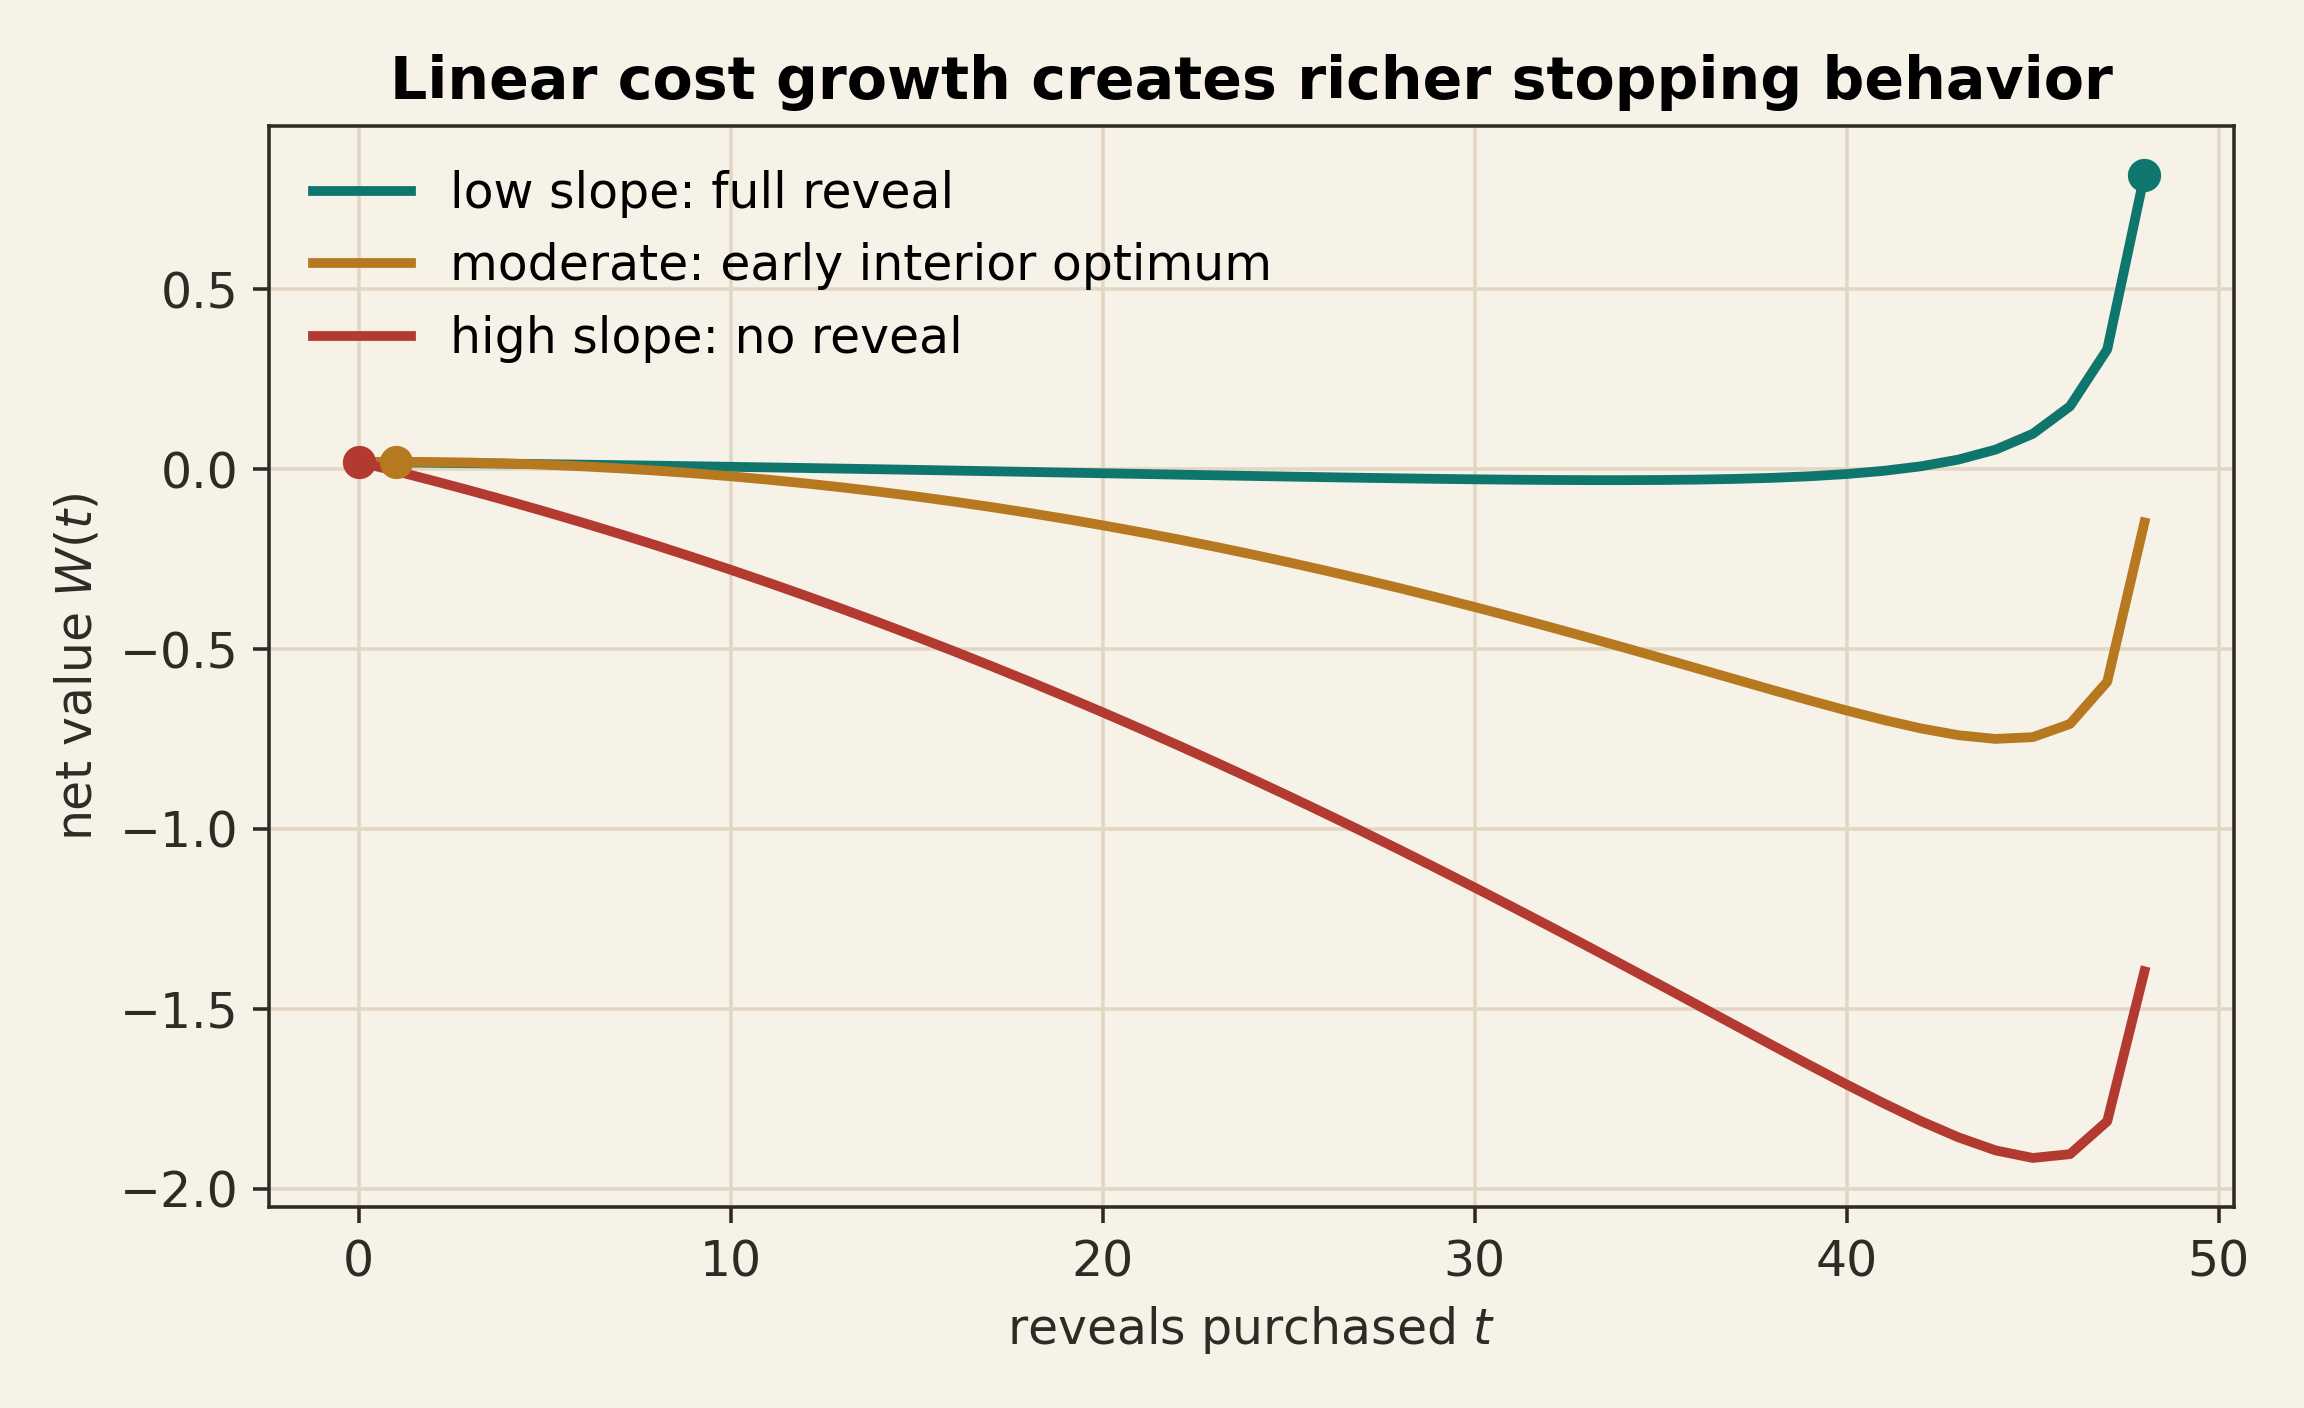
\includegraphics[width=0.88\linewidth]{fig_linear_regimes.png}
  \caption{With linearly increasing reveal costs $c_t=a+bt$, the optimum can
  occur at no reveal, at full reveal, or at an interior stopping time.}
  \label{fig:linear-regimes}
\end{figure}

\section{Linearly Increasing Costs}

Consider
\[
  c_t=a+bt,\qquad a,b\ge0.
\]
Then
\[
  W(t+1)-W(t)
  =
  \frac{m(K-1)}{K(K-2-t)(K-1-t)}-(a+bt).
\]
Both terms on the right can increase.  The benefit term rises slowly at first
and sharply near full revelation; the cost term rises steadily.  Their
difference can cross zero more than once, creating interior local maxima.

This gives a simple interpretation:

\begin{itemize}
\item If $a$ and $b$ are low, late information dominates and full reveal wins.
\item If $a$ is high, buying even the first reveal is unattractive.
\item If early costs are low but $b$ is high enough, the first few reveals
can be worthwhile while continued revealing becomes too expensive, producing
an interior optimum.
\end{itemize}

\begin{figure}[ht]
  \centering
  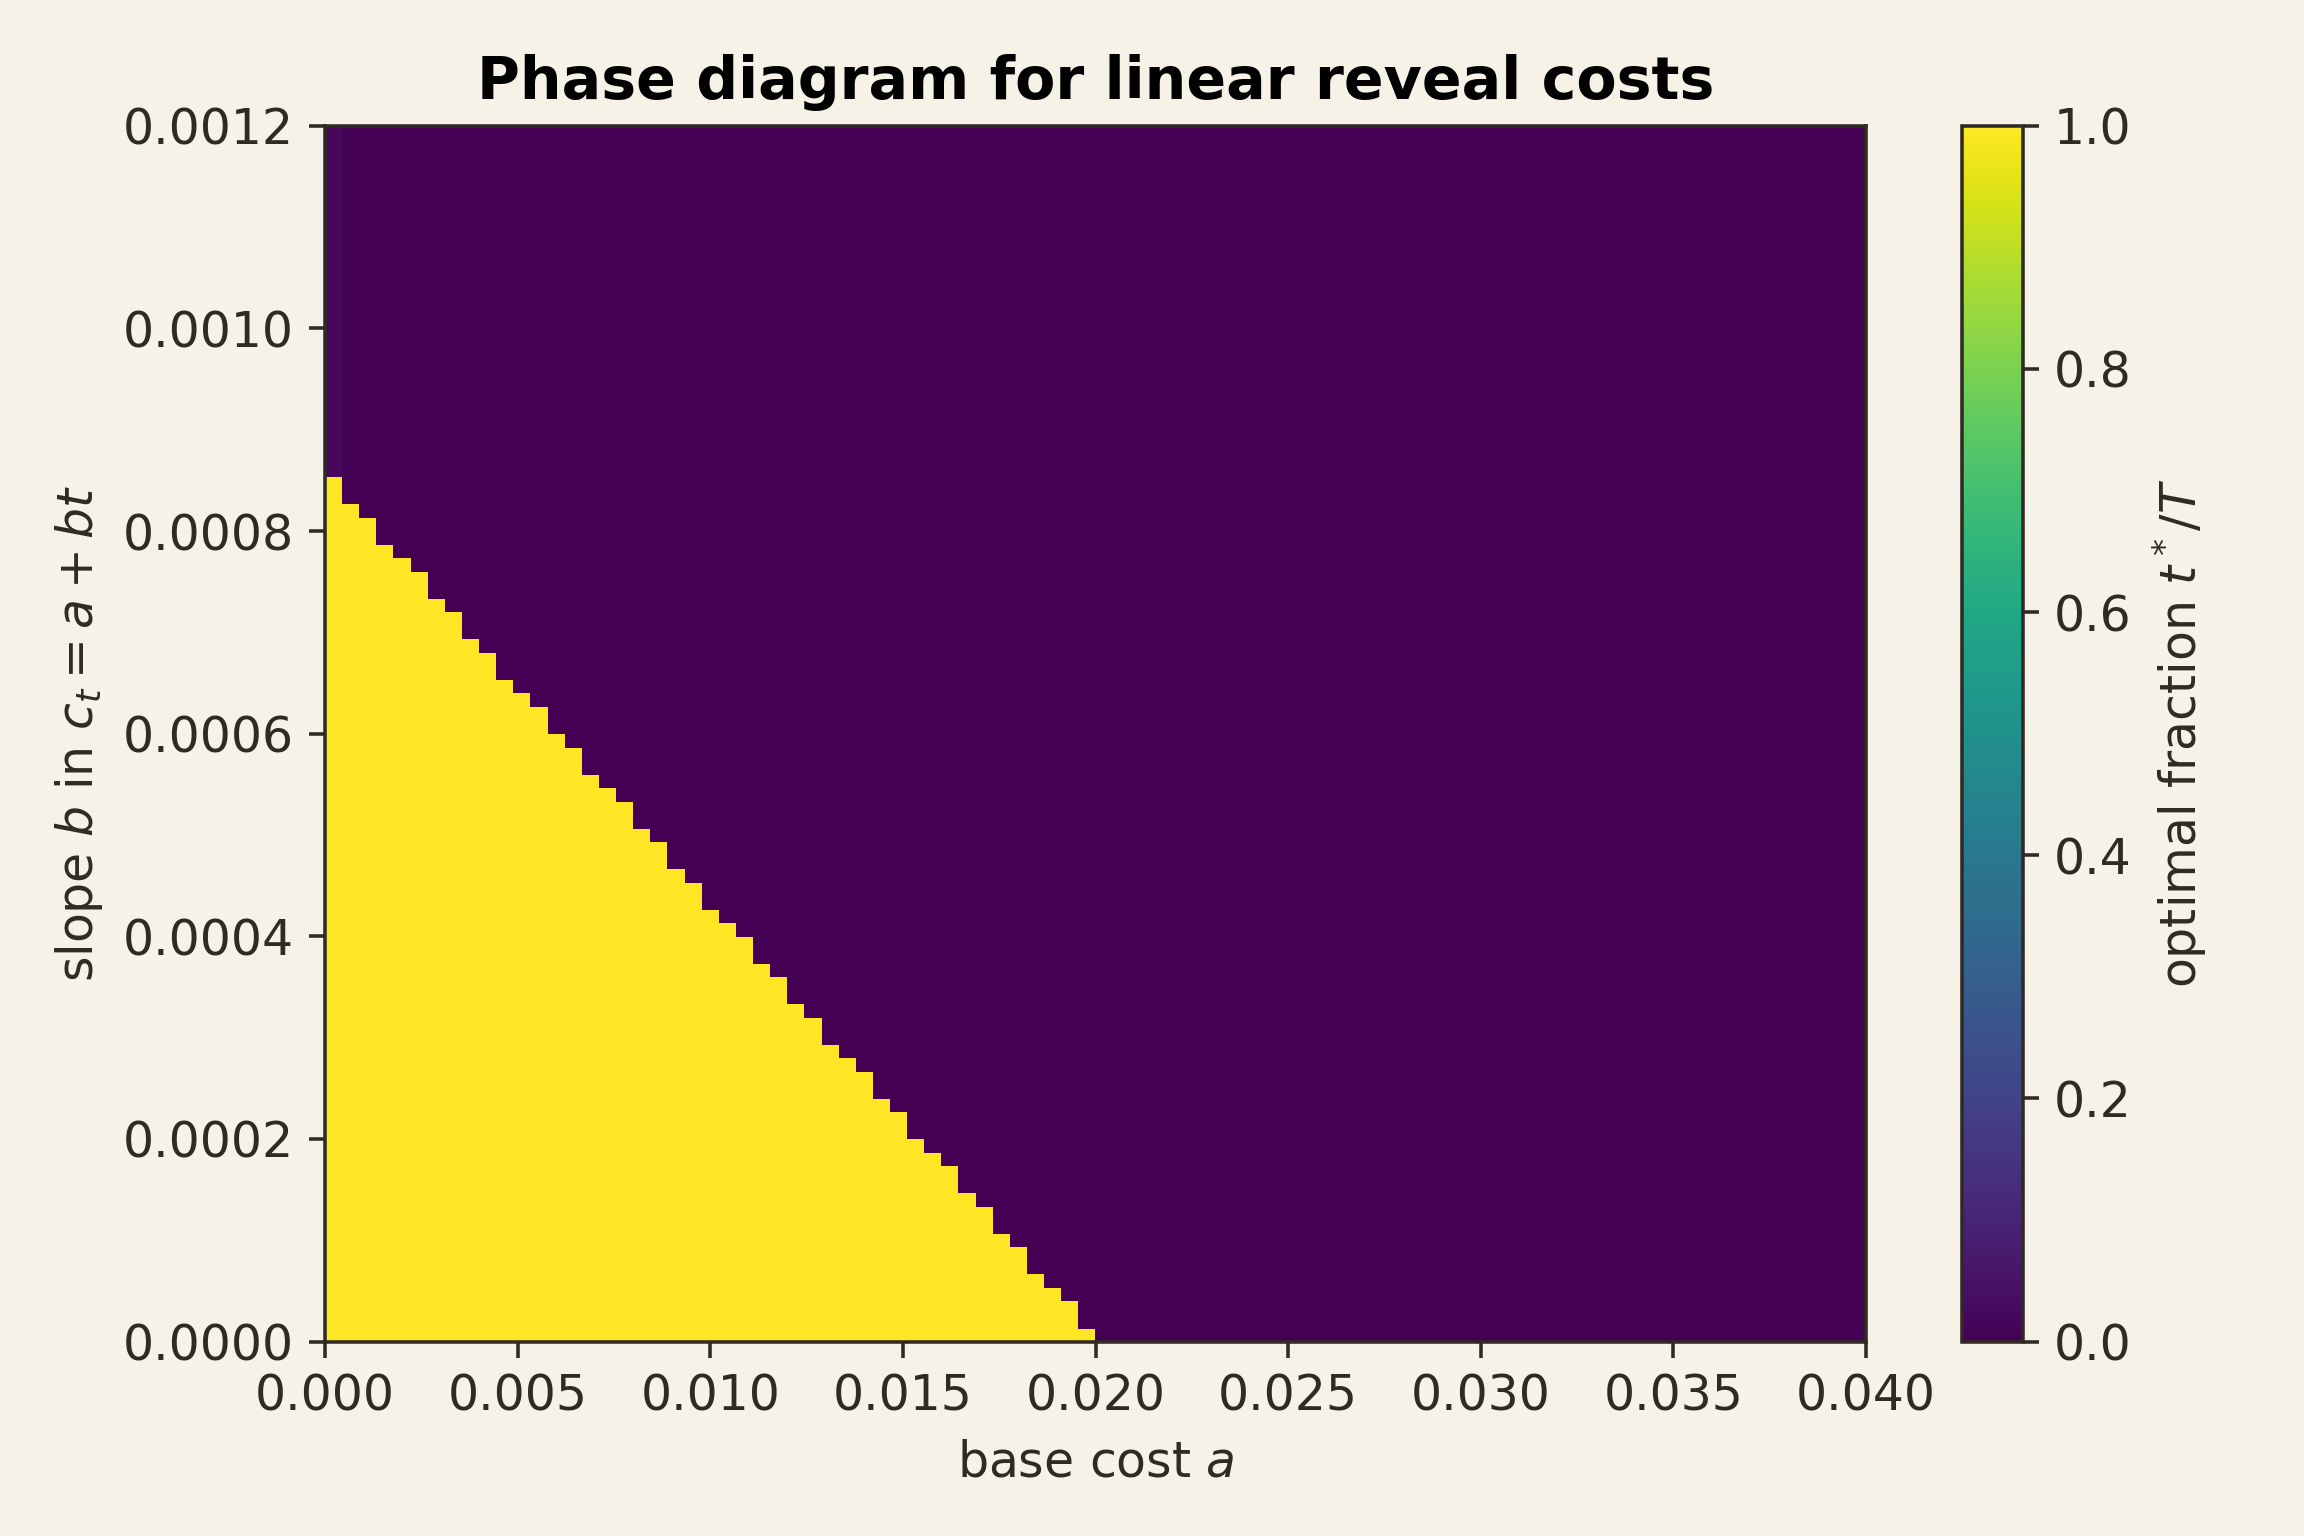
\includegraphics[width=0.88\linewidth]{fig_linear_phase.png}
  \caption{A phase diagram for $K=50,m=1$ and $c_t=a+bt$.  Color indicates
  the optimal fraction of possible reveals purchased.}
  \label{fig:linear-phase}
\end{figure}

\section{Costs That Rise and Then Saturate}

In many learning processes, costs rise early but do not rise forever.  There
may be setup costs, attention costs, or search-friction costs that plateau
once the process is underway.  Two simple forms are
\[
  c_t=a+\min\{bt,L\}
\]
and
\[
  c_t=a+L(1-e^{-t/\tau}).
\]
These costs initially increase, but eventually flatten.  Because $\Delta_t$
continues to rise sharply near the end, saturated costs can restore the
push-through effect: after paying through the early region, late reveals
become increasingly attractive again.

\begin{figure}[ht]
  \centering
  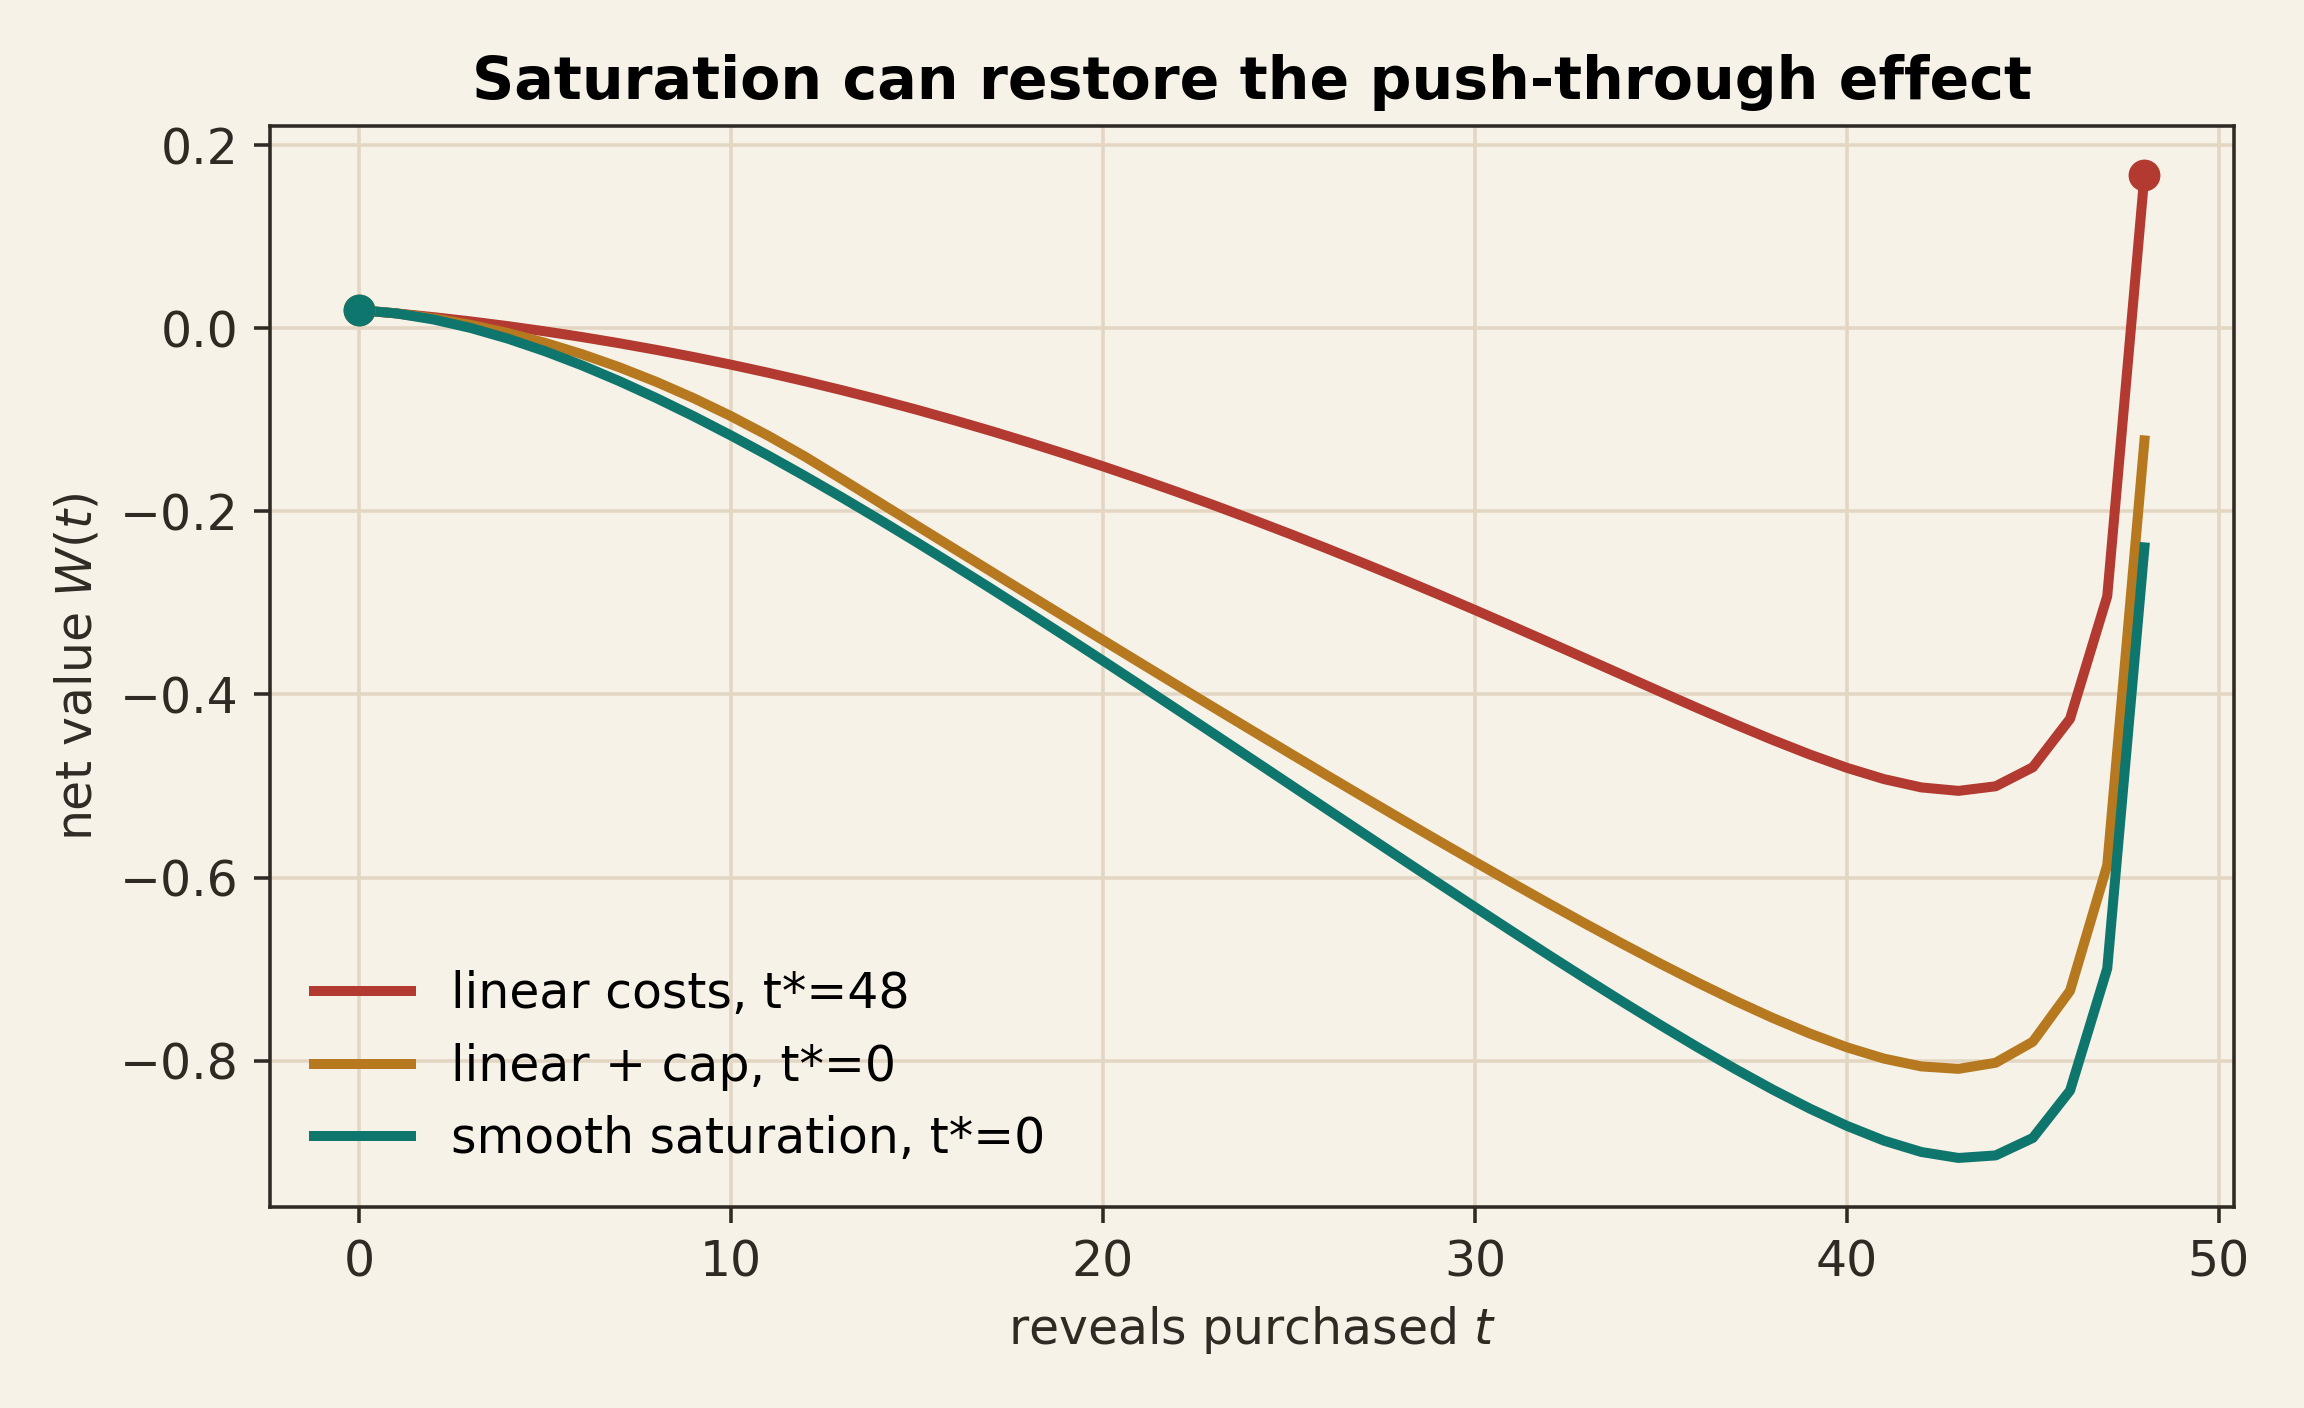
\includegraphics[width=0.88\linewidth]{fig_saturation_pushthrough.png}
  \caption{Compared with purely linear costs, saturating cost curves can make
  late-stage full revelation optimal again.}
  \label{fig:saturation-push}
\end{figure}

\begin{figure}[ht]
  \centering
  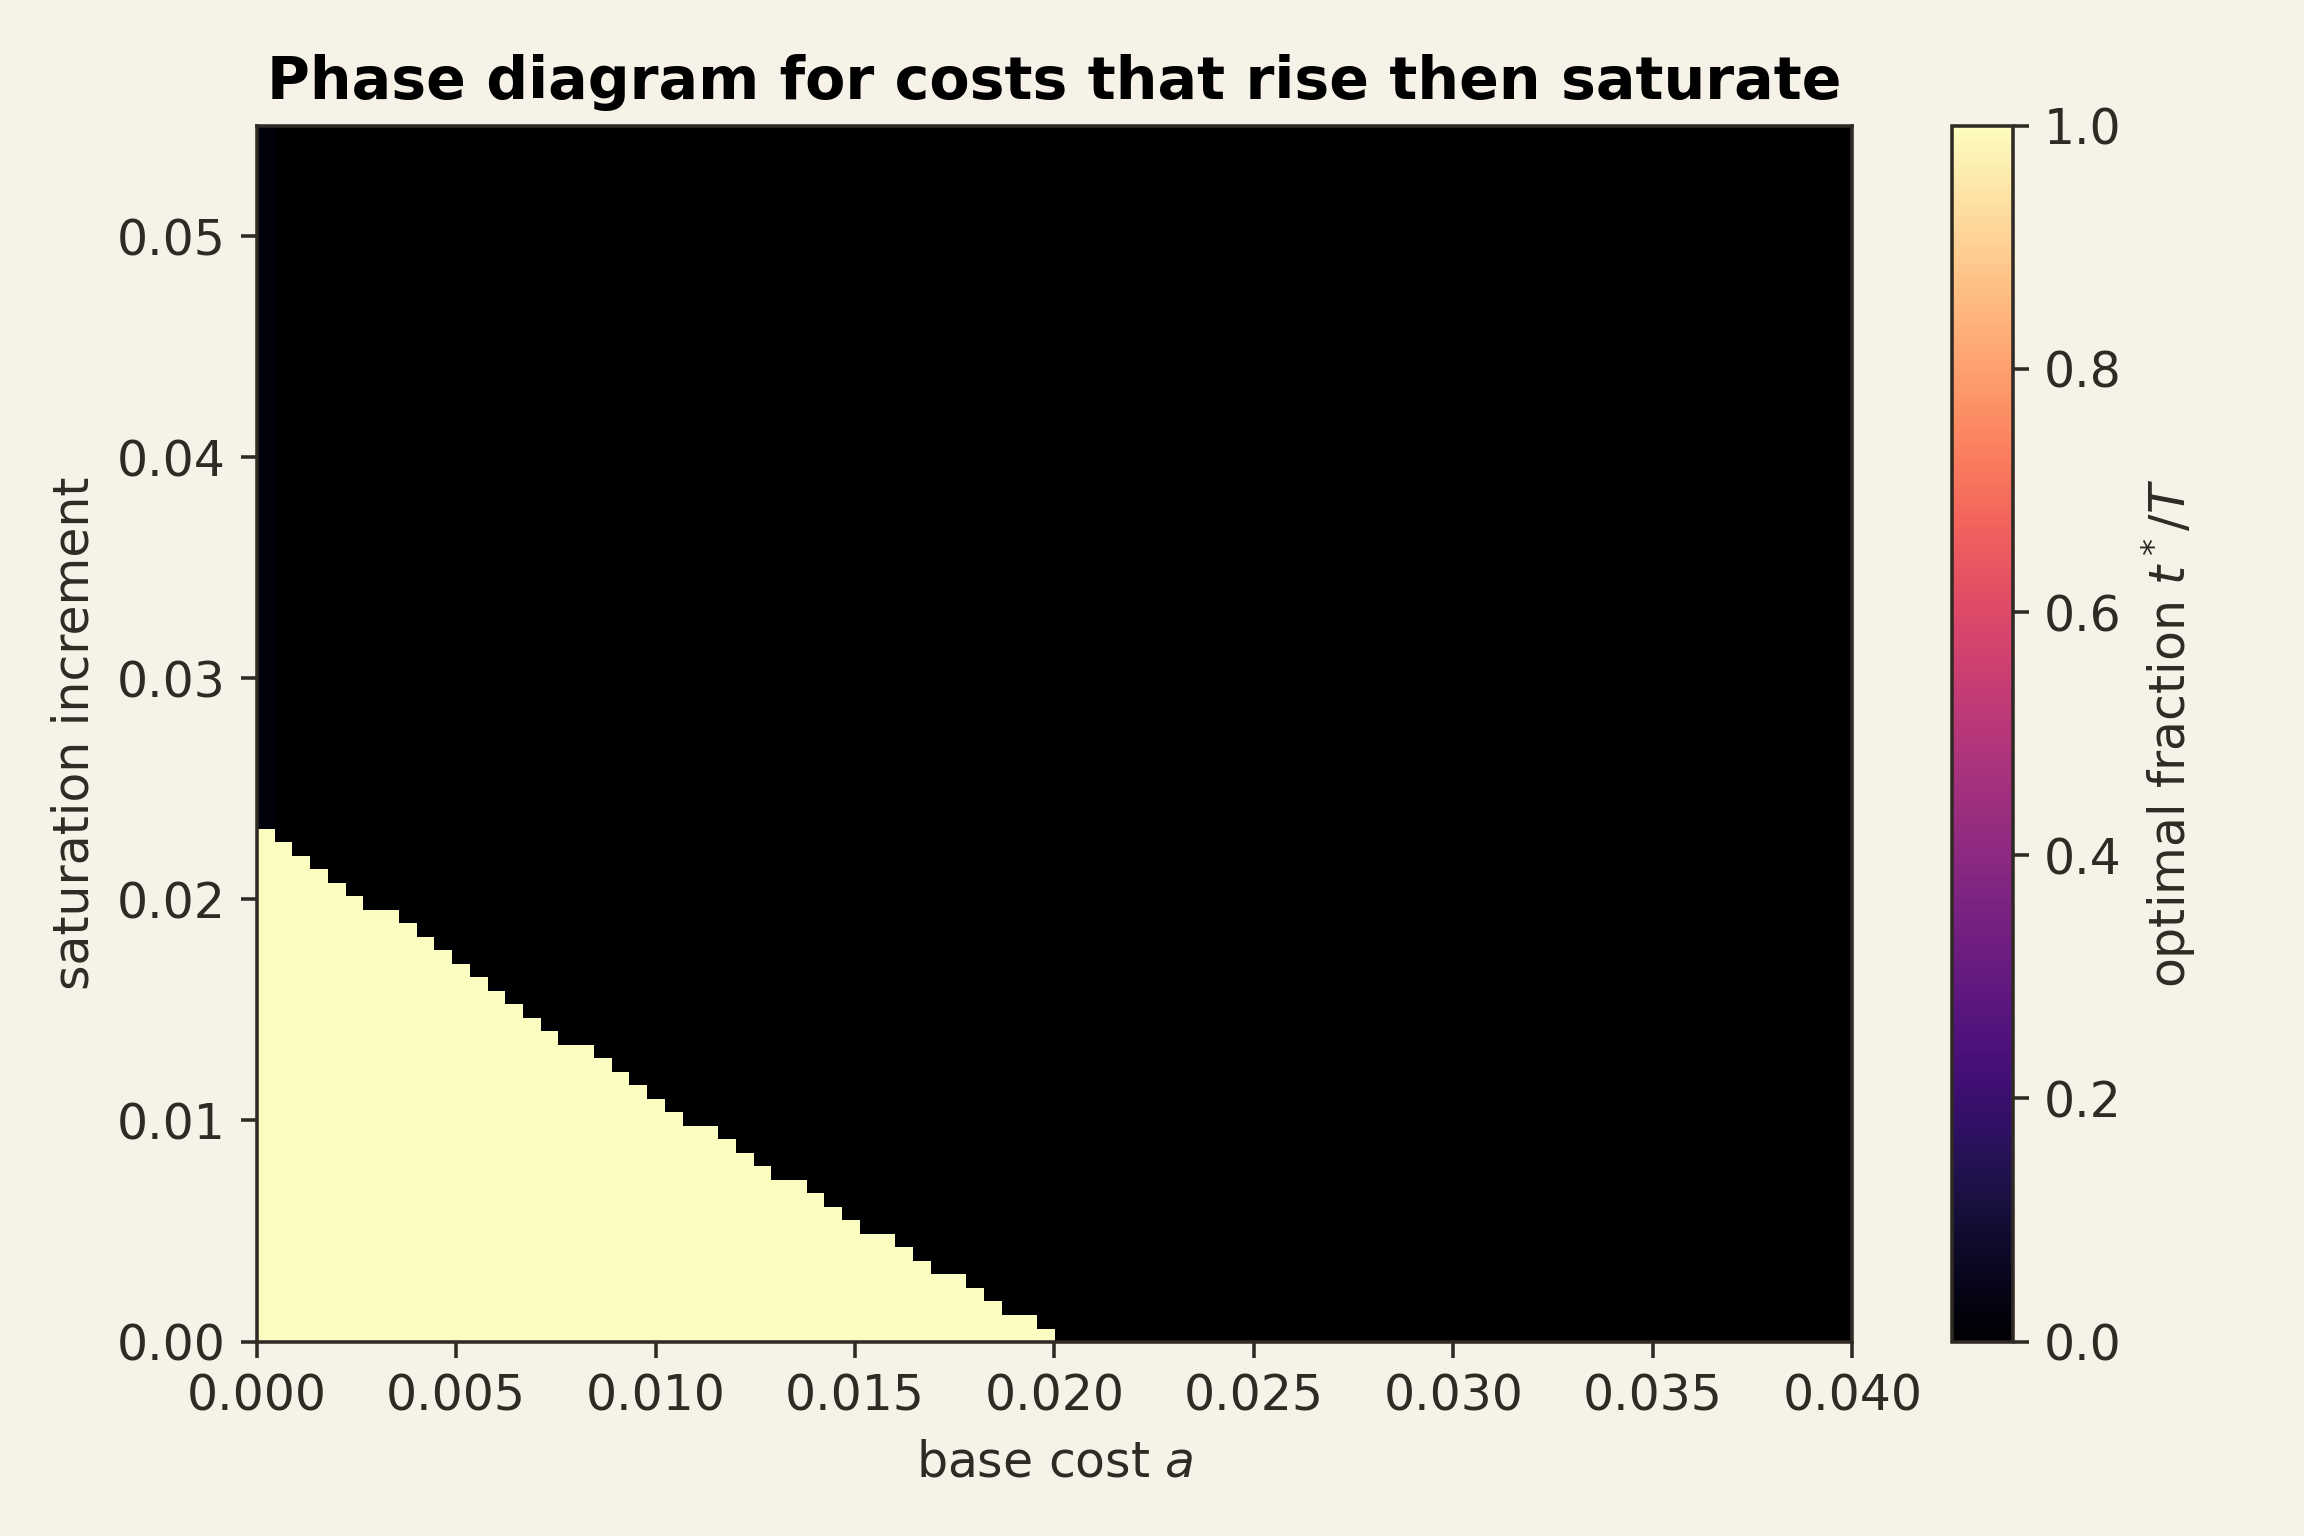
\includegraphics[width=0.88\linewidth]{fig_saturating_phase.png}
  \caption{A phase diagram for costs of the form $c_t=a+\min\{bt,L\}$, with
  fixed slope and varying base cost and saturation level.}
  \label{fig:saturating-phase}
\end{figure}

\section{Interpretation}

Variable costs separate two ideas that coincide in the constant-cost model.
The first idea is robust: eliminative information has increasing marginal
value.  The second idea is fragile: endpoint optimality.  Endpoint optimality
requires the net increments to have the right monotonic shape.  Constant costs
guarantee that shape; arbitrary variable costs do not.

The useful organizing principle is therefore not simply ``reveal everything
or reveal nothing.''  It is:
\[
  \hbox{continue when } \Delta_t \hbox{ is large relative to } c_t.
\]
Since $\Delta_t$ is back-loaded, the value of a reveal can be low early and
high late.  Whether the player reaches the high-value region depends on the
cost curve.

\section{Conclusion}

The exact $1/K$ threshold from Part I is a clean benchmark, but it is not the
end of the story.  Variable reveal costs generate a richer stopping geometry.
Linearly increasing costs can produce interior optima.  Costs that rise and
saturate can restore the Monty-style push-through effect.  Across these
variants, the central mechanism remains the same: eliminative information
concentrates probability mass, so its marginal value rises as the set of
remaining possibilities shrinks.

\end{document}
